%%%%%%%%%%%%%%%%%%%%%%%%%%%%%%%%%%%%%%%%%
% Masters/Doctoral Thesis 
% LaTeX Template
% Version 2.5 (27/8/17)
%
% This template was downloaded from:
% http://www.LaTeXTemplates.com
%
% Version 2.x major modifications by:
% Vel (vel@latextemplates.com)
%
% This template is based on a template by:
% Steve Gunn (http://users.ecs.soton.ac.uk/srg/softwaretools/document/templates/)
% Sunil Patel (http://www.sunilpatel.co.uk/thesis-template/)
%
% Template license:
% CC BY-NC-SA 3.0 (http://creativecommons.org/licenses/by-nc-sa/3.0/)
%
%%%%%%%%%%%%%%%%%%%%%%%%%%%%%%%%%%%%%%%%%

%----------------------------------------------------------------------------------------
%	PACKAGES AND OTHER DOCUMENT CONFIGURATIONS
%----------------------------------------------------------------------------------------

\documentclass[
11pt, % The default document font size, options: 10pt, 11pt, 12pt
oneside, % Two side (alternating margins) for binding by default, uncomment to switch to one side
english, % ngerman for German
% singlespacing, % Single line spacing, alternatives: onehalfspacing or doublespacing
% TODO - something is overrulling our doublespacing, need to find out what
onehalfspacing,
%draft, % Uncomment to enable draft mode (no pictures, no links, overfull hboxes indicated)
%nolistspacing, % If the document is onehalfspacing or doublespacing, uncomment this to set spacing in lists to single
%liststotoc, % Uncomment to add the list of figures/tables/etc to the table of contents
%toctotoc, % Uncomment to add the main table of contents to the table of contents
%parskip, % Uncomment to add space between paragraphs
%nohyperref, % Uncomment to not load the hyperref package
headsepline, % Uncomment to get a line under the header
%chapterinoneline, % Uncomment to place the chapter title next to the number on one line
consistentlayout, % Uncomment to change the layout of the declaration, abstract and acknowledgements pages to match the default layout
reqno, % align equation numbers to right
]{MastersDoctoralThesis} % The class file specifying the document structure

% This goes with setspace package
% \onehalfspacing

\usepackage[utf8]{inputenc} % Required for inputting international characters
\usepackage[T1]{fontenc} % Output font encoding for international characters

\usepackage{mathpazo} % Use the Palatino font by default - Lara Chammas used this one
% Looks time TNR so let's go with that
% \usepackage{newtxmath,newtxtext} % Times New Roman - the required type
% filler to get idea of formatting
\usepackage{lipsum}
% pdf pages for appending original project proposal
\usepackage{pdfpages}

\usepackage[backend=bibtex,style=authoryear,natbib=true]{biblatex} % Use the bibtex backend with the authoryear citation style (which resembles APA)

\addbibresource{dissertation.bib} % The filename of the bibliography

\usepackage[autostyle=true]{csquotes} % Required to generate language-dependent quotes in the bibliography

\usepackage{mathtools} % for floor symbol
%----------------------------------------------------------------------------------------
%	MARGIN SETTINGS
%----------------------------------------------------------------------------------------

\geometry{
	paper=a4paper, % Change to letterpaper for US letter
	inner=2.5cm, % Inner margin
	outer=2.5cm, % Outer margin
	% bindingoffset=.5cm, % Binding offset
	top=1.5cm, % Top margin
	bottom=1.5cm, % Bottom margin
	%showframe, % Uncomment to show how the type block is set on the page
}

%----------------------------------------------------------------------------------------
%	THESIS INFORMATION
%----------------------------------------------------------------------------------------

% Other possible titles
% 1. Keywords: detect, transparent, 3D Shape, Surface Normals, Manipulation, Robotics, Computer Vision
% 2. 
\thesistitle{Detecting transparent objects \\ with an RGB-D camera} % Your thesis title, this is used in the title and abstract, print it elsewhere with \ttitle
\supervisor{Artur Garcez} % Your supervisor's name, this is used in the title page, print it elsewhere with \supname
\examiner{} % Your examiner's name, this is not currently used anywhere in the template, print it elsewhere with \examname
\degree{Doctor of Philosophy} % Your degree name, this is used in the title page and abstract, print it elsewhere with \degreename
\author{Daniel Sikar} % Your name, this is used in the title page and abstract, print it elsewhere with \authorname
\addresses{} % Your address, this is not currently used anywhere in the template, print it elsewhere with \addressname

\subject{Biological Sciences} % Your subject area, this is not currently used anywhere in the template, print it elsewhere with \subjectname
\keywords{Autonomous Vehicles, Convolutional Neural Networks} % Keywords for your thesis, this is not currently used anywhere in the template, print it elsewhere with \keywordnames
\university{City, University of London} % Your university's name and URL, this is used in the title page and abstract, print it elsewhere with \univname
\department{\href{http://department.university.com}{Department or School Name}} % Your department's name and URL, this is used in the title page and abstract, print it elsewhere with \deptname
\group{\href{http://researchgroup.university.com}{Research Group Name}} % Your research group's name and URL, this is used in the title page, print it elsewhere with \groupname
\faculty{\href{http://faculty.university.com}{Faculty Name}} % Your faculty's name and URL, this is used in the title page and abstract, print it elsewhere with \facname

\AtBeginDocument{
\hypersetup{pdftitle=\ttitle} % Set the PDF's title to your title
\hypersetup{pdfauthor=\authorname} % Set the PDF's author to your name
\hypersetup{pdfkeywords=\keywordnames} % Set the PDF's keywords to your keywords
\hypersetup{hidelinks}
}

% do not indent paragraphs
\setlength\parindent{0pt}
% Add 
\setlength{\parskip}{0.5em} % changes vertical space between paragraphs, alternatively use pt unit e.g. {10pt} %
% Appendix
\usepackage{appendix}

\begin{document}

\frontmatter % Use roman page numbering style (i, ii, iii, iv...) for the pre-content pages

\pagestyle{plain} % Default to the plain heading style until the thesis style is called for the body content

%----------------------------------------------------------------------------------------
%	TITLE PAGE
%----------------------------------------------------------------------------------------

\begin{titlepage}
\begin{center}

\vspace*{.06\textheight}
{\scshape\LARGE \univname\par}\vspace{1.5cm} % University name
\textsc{\Large MSc in Data Science}\\[0.5cm] % Thesis type
\textsc{\Large Project Report}\\[0.5cm]
\textsc{\Large 2020}\\[0.5cm]

\HRule \\[0.4cm] % Horizontal line
{\huge \bfseries \ttitle\par}\vspace{0.4cm} % Thesis title
\HRule \\[3.5cm] % Horizontal line
 
% \begin{minipage}[t]{0.4\textwidth}
\begin{flushleft} \large
% \emph{Author:}\\
\authorname \\ [1cm]
%\href{http://www.johnsmith.com}{\authorname} % Author name - remove the \href bracket to remove the link
% \end{flushleft}
% \end{minipage}
% \begin{minipage}[t]{0.4\textwidth}
% \begin{flushright} \large

\emph{Supervised by:} 
\supname \\ [3.5cm] % Supervisor name - remove the \href bracket to remove the link  
\end{flushleft}
% \end{flushright}
%\end{minipage}\\[3cm]
 

%\large \textit{A thesis submitted in fulfillment of the requirements\\ for the degree of %\degreename}\\[0.3cm] % University requirement text
%\textit{in the}\\[0.4cm]
%\groupname\\\deptname\\[2cm] % Research group name and department name
 

{\large \today}\\[4cm] % Date
%\includegraphics{Logo} % University/department logo - uncomment to place it
 
%vfill
\end{center}
\end{titlepage}

%----------------------------------------------------------------------------------------
%	DECLARATION PAGE
%----------------------------------------------------------------------------------------

%%%%%%%%%%%%%%%%%
%% DECLARATION %%
%%%%%%%%%%%%%%%%%

\begin{declaration}
\addchaptertocentry{\authorshipname} % Add the declaration to the table of contents
\noindent By submitting this work, I declare that this work is entirely my own except those parts duly identified and referenced in my submission. It complies with any specified word limits and the requirements and regulations detailed in the assessment instructions and any other relevant programme and module documentation. In submitting this work I acknowledge that I have read and understood the regulations and code regarding academic misconduct, including that relating to plagiarism, as specified in the Programme Handbook. I also acknowledge that this work will be subject to a variety of checks for academic misconduct. \\[1cm]
 
\noindent Signed:\\[1cm]
\authorname 
%Daniel Sikar
%\rule[0.5em]{25em}{0.5pt} % This prints a line for the signature
 
%\noindent Date:\\
%\rule[0.5em]{25em}{0.5pt} % This prints a line to write the date
\end{declaration}

\cleardoublepage

% \begin{declaration}
% \addchaptertocentry{\authorshipname} % Add the declaration to the table of contents
%\noindent By submitting this work, I declare that this work is entirely my own except those parts duly identified and referenced in my submission. It complies with any specified word limits and the requirements and regulations detailed in the assessment instructions and any other relevant programme and module documentation. In submitting this work I acknowledge that I have read and understood the regulations and code regarding academic misconduct, including that relating to plagiarism, as specified in the Programme Handbook. I also acknowledge that this work will be subject to a variety of checks for academic misconduct. \\[1cm]
 
%\noindent Signed:\\[1cm]
%Daniel Sikar
%\rule[0.5em]{25em}{0.5pt} % This prints a line for the signature
 
%\noindent Date:\\
%\rule[0.5em]{25em}{0.5pt} % This prints a line to write the date
%\end{declaration}

\cleardoublepage

%----------------------------------------------------------------------------------------
%	QUOTATION PAGE
%----------------------------------------------------------------------------------------

%\vspace*{0.2\textheight}

%\noindent\enquote{\itshape Thanks to my solid academic training, today I can write hundreds of words on virtually any topic without possessing a shred of information, which is how I got a good job in journalism.}\bigbreak

%\hfill Dave Barry

%----------------------------------------------------------------------------------------
%	ABSTRACT PAGE
%----------------------------------------------------------------------------------------

%%%%%%%%%%%%%%
%% ABSTRACT %%
%%%%%%%%%%%%%%

%From INM363 MSc Project Guidance Document 2019-20:  

%1. You are expected to clearly identify a problem or requirement, justifying why it is worth exploring or implementing, develop a method suitable for the work, apply this method, analyse the results and evaluate their implications.  

%2. Page 2 must contain an indicative Abstract of 100-200 words, and up to five keywords. This is more than an introduction to the project – it should explain what has been achieved and how

\begin{abstract}
\addchaptertocentry{\abstractname} % Add the abstract to the table of contents
Clear-object detection, e.g. glass and transparent plastic, with depth cameras present challenges inherent to the physical aspects of material such as opacity and consequently diffused and reflected light. As depth cameras rely on laser 

\vspace{25mm} %25mm vertical space
  
  
\textbf{Keywords:} keyword1, keyword2, keyword3

\end{abstract}

%----------------------
%	ACKNOWLEDGEMENTS
%----------------------

%\begin{acknowledgements}
%\addchaptertocentry{\acknowledgementname} % Add the acknowledgements to the table of contents
%The acknowledgments and the people to thank go here, don't forget to include your project %advisor\ldots
%\end{acknowledgements}

%----------------------------------------------------------------------------------------
%	LIST OF CONTENTS/FIGURES/TABLES PAGES
%----------------------------------------------------------------------------------------

\tableofcontents % Prints the main table of contents

% \listoffigures % Prints the list of figures

% \listoftables % Prints the list of tables

%----------------------------------------------------------------------------------------
%	ABBREVIATIONS
%----------------------------------------------------------------------------------------

%\begin{abbreviations}{ll} % Include a list of abbreviations (a table of two columns)

%\textbf{LAH} & \textbf{L}ist \textbf{A}bbreviations \textbf{H}ere\\
%\textbf{WSF} & \textbf{W}hat (it) \textbf{S}tands \textbf{F}or\\

%\end{abbreviations}

%----------------------------------------------------------------------------------------
%	PHYSICAL CONSTANTS/OTHER DEFINITIONS
%----------------------------------------------------------------------------------------

%\begin{constants}{lr@{${}={}$}l} % The list of physical constants is a three column table

% The \SI{}{} command is provided by the siunitx package, see its documentation for instructions on how to use it

%Speed of Light & $c_{0}$ & \SI{2.99792458e8}{\meter\per\second} (exact)\\
%Constant Name & $Symbol$ & $Constant Value$ with units\\

%\end{constants}

%----------------------------------------------------------------------------------------
%	SYMBOLS
%----------------------------------------------------------------------------------------

%\begin{symbols}{lll} % Include a list of Symbols (a three column table)

%$a$ & distance & \si{\meter} \\
%$P$ & power & \si{\watt} (\si{\joule\per\second}) \\
%Symbol & Name & Unit \\

%\addlinespace % Gap to separate the Roman symbols from the Greek

%$\omega$ & angular frequency & \si{\radian} \\

%\end{symbols}

%----------------------------------------------------------------------------------------
%	DEDICATION
%----------------------------------------------------------------------------------------

% \dedicatory{For/Dedicated to/To my\ldots} 

%----------------------------------------------------------------------------------------
%	THESIS CONTENT - CHAPTERS
%----------------------------------------------------------------------------------------

\mainmatter % Begin numeric (1,2,3...) page numbering

\pagestyle{thesis} % Return the page headers back to the "thesis" style

% Include the chapters of the thesis as separate files from the Chapters folder
% Uncomment the lines as you write the chapters

%\include{Chapters/Chapter1}
%%%%%%%%%%%%%%%%%%%%%%%%%%%%%%%%%
%% INTRODUCTION AND OBJECTIVES %%
%%%%%%%%%%%%%%%%%%%%%%%%%%%%%%%%%

%This chapter should set the scene for the reader. It must outline the background to the problem, give your reasons for the choice of project, and identify the project’s beneficiaries. Your objectives need to be precisely stated, together with the tests that will show, at the end of the project, that they have been met (or not been met). You need also to outline your methods in broad terms, along with y work plan with sufficient detail to show how you planned to meet the objectives. Outline any major changes of goals or methods that happened during the project. Finally, outline the structure of the report, showing how it fits together.

\chapter{Introduction and Objectives}
\label{Intro} 
\lipsum[1]

%-----------------------------------
%	BACKGROUND
%-----------------------------------

\section{Background}
\lipsum[1]

%-----------------------------------
%	AIMS AND OBJECTIVES
%-----------------------------------

\section{Aims and Objectives}
\lipsum[1]


%-----------------------------------
%	BENEFICIARIES
%-----------------------------------

\subsection{Beneficiaries}
\lipsum[1]

%-----------------------------------
%	METHODS AND WORKPLAN
%-----------------------------------

\section{Introduction to Methods and Workplan}
\lipsum[1]

%-----------------------------------
%	CHANGES IN METHODS AND WORKPLAN
%-----------------------------------

\subsection{Changes in Methods and Workplan}
\lipsum[1]


%-----------------------------------
%	REPORT STRUCTURE
%-----------------------------------

\section{Structure of the Report}
\lipsum[1]





 
%%%%%%%%%%%%%
%% CONTEXT %%
%%%%%%%%%%%%%

%This chapter explains the current state of your topic, in practice and theory. This is the state of the world which you intend to improve, and the state of knowledge on top of which you build your advances and from which you learn knowledge to apply and constraints on your work. So, you will report and analyse what is known about a certain topic, as reported in reference literature and published scientific literature; if you are developing a product, you will need to report about comparable or competing products over which you intend to improve or from which you will obtain ideas; you may need to describe legal or societal situation within which your work takes place; etc.  
  
%It is important to demonstrate scholarship, i.e. the ability to read about a subject area in a range of sources, assimilate the material and then discuss it intelligently.  
  
%You should demonstrate that you understand what you have read by providing some analysis or commentary in view of the goals of your project: it is not enough simply to provide summaries of what you have read. References should be cited following the Harvard Referencing Style. You must also explain, both in this chapter and, as appropriate, in others, how the results of the studies to which you make reference inform your project work. To gain a passing grade, your report MUST demonstrate adequate engagement with academic literature and any other sources necessary for the work to be well informed.  

% The story we want to tell
% (...)

\chapter{Context}
\label{Context} 

"Transparent objects are a common part of everyday life, yet they possess unique visual properties that make them incredibly difficult for standard 3D sensors to produce accurate depth estimates for. In many cases, they often appear as noisy or distorted approximations of the surfaces that lie behind them. To address these challenges, we present ClearGrasp -- a deep learning approach for estimating accurate 3D geometry of transparent objects from a single RGB-D image for robotic manipulation. Given a single RGB-D image of transparent objects, ClearGrasp uses deep convolutional networks to infer surface normals, masks of transparent surfaces, and occlusion boundaries. It then uses these outputs to refine the initial depth estimates for all transparent surfaces in the scene. To train and test ClearGrasp, we construct a large-scale synthetic dataset of over 50,000 RGB-D images, as well as a real-world test benchmark with 286 RGB-D images of transparent objects and their ground truth geometries. The experiments demonstrate that ClearGrasp is substantially better than monocular depth estimation baselines and is capable of generalizing to real-world images and novel objects. We also demonstrate that ClearGrasp can be applied out-of-the-box to improve grasping algorithms' performance on transparent objects." \cite{sajjan2019cleargrasp}.

RGB-D cameras.

\cite{RakhimkulEtAl2019} Assistive robot solutions are mostly designed as robot helpers with robotic arms and aim to assist disabled and elderly people with carrying out basic activities of daily life such as reaching household objects, i.e. cups, feeding with spoon,opening a drawer/fridge doors, etc., However, commercial assistive robotic arms with joystick control require extensive and tiring hand motor skill training that limits robot’s practical usage by patients with disabilities. The main objective of this work is to present the methodology for designing an intelligent human-machine interface for a commercial joystick controlled assistive robotic arm realizing shared autonomy and supervisory control modes. Preliminary results on a RGB-D based object detection and position estimation system development using publicly available YOLOv3 and CenterNet deep learning models implementation of an autonomous object grasping mode by the Kinova Jaco robotic arm are described in detail and experimentally demonstrated.

\cite{batzner2021se3equivariant} guys say that small datasets work ok.\cite{power2021simple} also found this, and \cite{vu2021machine}. These guys \cite{frankle2019lottery} discuss small networks

% Conferences

% https://www.mhnetwork.com/conference-on-collaborative-robots-advanced-vision-and-artificial-intelligence/

%-----------------------------------
%	RELATED WORK
%-----------------------------------

\section{Related Work}
\label{context:related-work} 
TODO There should be plenty on the cleargrasp paper, plus other references following up/down the reference tree. At this point we could use scholarly and semantic scholar
% https://github.com/dsikar/scholarly

\lipsum[1]







%%%%%%%%%%%%%
%% METHODS %%
%%%%%%%%%%%%%

%This chapter describes in detail the methods for whatever activities were necessary for your project – e.g., data gathering, data analysis, requirements analysis, design, implementation, testing/evaluation, etc. Your choice of methods should be discussed and justified in view of the project objectives, and with reference to the pertinent literature. Report not only what methods you applied in generic terms, but what you actually did: sufficient information about dates and details for your reader to understand how you ran your project, rather than just how one could run any similar project. 

\chapter{Methods}
\label{Methods} 

This chapter describes the methods used to generate the prediction model.

%-----------------------------------
%	AUTOENCODERS
%-----------------------------------

\section{Autoencoders}

% maybe best moved conda, ros, unity, etc (i.e. plumbing) to appendix, and keep here only the specific network architectures, cameras and camera libraries.

\section{conda}

% https://docs.conda.io/projects/conda/en/latest/index.html

conda (\cite{Conda2021}) is a system that simplifies package management and deployment. It is part of the Anaconda Python distribution. conda allows environments to be created, saved and switched from one to another, such that separate environments can be configured and run. A list of conda commands used in this project is given in \ref{app_methods:conda}. While conda can act as a package installer, it is only used here as an environment manager, while pip is used a a package manager.

\section{pip}

pip (\cite{pip2021}) is a package installer for Python that can be used to install packages from PyPI (the Python Package Index), a repository for the Python programming language, used to distribute software written in Python.

\section{UR3}
% https://www.universal-robots.com/products/ur3-robot/

The original experiment used a UR3 robotic arm
% Tinker Braccio - max load 150g
% https://store.arduino.cc/tinkerkit-braccio-robot
% will probably have to go with that plus a wall mount scenario
% https://www.zivid.com/zivid-one-plus
% SDKs
% https://www.zivid.com/downloads

%%%%%%%%%%%%%%%
% SETUP
%%%%%%%%%%%%%%%
% Hardware
% 1. Zivid One+ camera in fixed position
% 2. Robotic Arm TBA
% 3. Transparent, translucent and opaque object

% Software
% 1. Tensorflow/Keras
% 2. ROS
% 3. Unity

% Models
% 1. Trained network for object detection
% 2. Trained network for path planning / object grasping
% 3. Trained network for command speech recognition - NTH

% All image and path planning data to be generated by Unity
% All audio data to be generated by GAN-like architectures, from a few audio samples

\section{Zivid One+}

\section{Niryo One}
% Train end-to-end to pick-and-place ? :D

% The story we are trying to tell
% 1. We'll retrieve an image RBD + RGBD from camera
% 2. The image x2 goes through a pipeline where the output is a prediction of the 3D space and objects present
% 3. A voice issues a command like move object from A to B
% 4. The 3D space and command are fed to another pipeline, which outputs a path
% the robotic arm needs to follow to move an object from location A to location B
\section{ROS}

\section{ROS x Arduino}

% https://maker.pro/arduino/tutorial/how-to-use-arduino-with-robot-operating-system-ros

% http://wiki.ros.org/rosserial_arduino/Tutorials

\section{Unity}
% Robotics' simulation in Unity
% https://resources.unity.com/unitenow/onlinesessions/simulating-robots-with-ros-and-unity

% Niryo One Robotic Arm in Unity
% https://blogs.unity3d.com/2020/11/19/robotics-simulation-in-unity-is-as-easy-as-1-2-3/

% ROS#
% https://github.com/siemens/ros-sharp

\section{Network Architectures}

In this section we discuss the network architectures used by ClearGrasp and Depth2Depth.



\section{Depth Cameras}

\begin{verbatim}
Start here: https://www.intelrealsense.com/beginners-guide-to-depth/
and take it from there.
Maybe also have a look here:
https://ulir.ul.ie/bitstream/handle/10344/7592/Sivcev_2018_Smart.pdf?sequence=5
Point GrayBumblebee 2 stereo camera
Point Gray BlackFly monocular camera
\end{verbatim}


\section{Prediction Workflow}

\begin{verbatim}
1. Input
2. Networks

eval_depth_completion.py, line 169:

We get the "corrected" output depth likesuch:

output_depth, filtered_output_depth = depthcomplete.depth_completion(
(...)

depth_completion is a method of the DepthToDepthCompletion class,
defined in:

depth_completion_api.py, line 732:
    def depth_completion(self,
    (...)
    which returns numpy arrays:
    
        return self.output_depth, self.filtered_output_depth

Note, these are to compute error metrics, the actual images
are stored during the inference process.

To obtain the two arrays:    
    # perform object segmentation
    def _modify_depth_delete_masks(

 571       self.mask_predicted = self.inferenceMasks.runOnNumpyImage
 
 
 _complete_depth
 
 # SURFACE NORMALS
 (...) self.inferenceNormals.runOnNumpyImage(input_image)
 
 Then, perform boundary detection:
 # OUTLINES
        self.occlusion_weight, self.occlusion_weight_rgb, self.outlines_rgb = self.inferenceOutlines.runOnNumpyImage(
            input_image)
            
            
 
 self.InferenceMasks
 
 3 models
 inference_models.InferenceNormals
 inference_models.InferenceOutlines(
 inference_models.InferenceMasks(
 
In inference_models.py:
 
self.model = deeplab_masks.DeepLab(num_classes=3, backbone='resnet', sync_bn=True,
                            freeze_bn=False)
                            
we get deeplab_masks from

from .modeling import deeplab, deeplab_masks

Network architectures used by each task (normal estimation, boundary detection and 
transparent object segmentation).

InferenceOutlines -> deeplab_resnet

InferenceNormals -> deeplab_resnet

InferenceMasks -> drn

In all three cases, image is presented as an one-dimensional array.
(...)
# Create Transforms
        self.transform = iaa.Sequential([
(...)


\end{verbatim}

\section{OpenEXR}
\begin{verbatim}
https://www.openexr.com/index.html - need a citation

https://scholar.google.com/scholar?hl=en&as_sdt=0%2C5&q=openexr+image+file+format&btnG=&oq=openexr
\end{verbatim}

OpenEXR is not playing well with windows. TODO Try on Ubuntu. Works ok on Ubuntu.

\section{deep2depth}
% from https://arxiv.org/pdf/1803.09326.pdf
"Overall,  our  main  algorithmic  insight  is  that  it  is  bestto  decompose  RGB-D  depth  completion  into  two  stages:1) prediction of surface normals and occlusion boundariesonly from color, and 2) optimization of global surface struc-ture from those predictions with soft constraints providedby observed depths.  During experiments we find with thisproposed  approach  has  significantly  smaller  relative  errorthan alternative approaches. It has the extra benefit that thetrained network is independent of the observed depths andso does not need to be retrained for new depth sensors."  
The one we are interested in are autoenconders and GAN architectures (citations 70 and 58, respectively).





%%%%%%%%%%%%%
%% RESULTS %%
%%%%%%%%%%%%%

%This chapter presents the outputs that you produced, by applying the methods that you have selected, including e.g. analysis, design, prototyping, experimental work, evaluation, etc.  
  
%How you report these results will depend on the nature of the work. It may be helpful to divide them into basic data (e.g., for a project that developed a software product, requirements specification, test data, etc.) and analysis of the data (e.g. statistical analyses, evaluation analyses, etc.). Remember that you are informing the reader of what you have produced and found and emphasising the interesting parts, 
% IMPORTANT - ADD SUMMARIES
% so summarising at the end of each major section is useful.  
  
%It is usually very helpful for the readers to include graphics and diagrams, for instance to clarify software design or requirements, identify key trends and relationships in empirical data, etc. If you do so, be sure to refer to these figures in the text and use them as evidence to support what you are explaining or arguing; and be sure that your figures are well designed and clearly presented – do not just use default settings of the software you are using in producing them.  
  
%It is essential that you identify clearly what you accomplished or produced yourself, as opposed to what existed before you started your individual project or was provided by others. For instance, some projects build new software on top of an existing code base, add new data to an existing body of data, or are executed by a student as a member of a team. It is essential to indicate what parts of the activities and results which you report are your own work. If this is left unclear, the markers are instructed not to give credit for work that they cannot attribute to you. Ambiguity would attract penalties for poor academic practice, with delays caused by any investigation (deception would be treated as academic misconduct, of course, which may lead to expulsion).

\chapter{Results}
\label{Results} 

\lipsum[1]
%%%%%%%%%%%%%%%%
%% DISCUSSION %%
%%%%%%%%%%%%%%%%

%This chapter examines your results in comparison with your objectives, and then in the wider perspective of other theoretical and applied work relevant to your project, as covered in your review in Chapter 2. For instance, for a software product you will discuss how well it satisfies the user needs that it addresses, its performance and dependability, aspects of design, implementation or assessment that have proved good choices or that instead you would change if you were to repeat the project knowing what you now know. For novel research results or any other knowledge obtained through the project, you will discuss your confidence in the results, their validity, scope and their generalisability. What are the implications of what you have found out? Do you have any recommendations as a result?

\chapter{Discussion}
\label{Discussion} 


%%%%%%%%%%%%%%%%%%%%%%%%%%%%%%%%%%%%%%%%%%%%
% EVALUATION, REFLECTIONS AND CONCLUSIONS %%
%%%%%%%%%%%%%%%%%%%%%%%%%%%%%%%%%%%%%%%%%%%%

%This chapter should evaluate the project work as a whole. Here the original choice of objectives, the literature examined, the methods used, the planning, etc. are all reviewed to see what has been achieved by undertaking the project. There may be a summary of general conclusions drawn from the work done, highlighting the particular contribution of your project. You should also consider the implications of these conclusions. Discuss any proposals that you might make for further work, having discovered what you now know. It is also important to include a reflective section covering what you have learned from the project process. What would you do differently if you were to start again, knowing what you now know? Your report MUST include adequate Evaluation, Reflections and Conclusions to gain a passing grade. 

\chapter{Evaluation, Reflections and Conclusions}
\label{Eval}



%----------------------------------------------------------------------------------------
%	BIBLIOGRAPHY
%----------------------------------------------------------------------------------------

\printbibliography[heading=bibintoc]

%----------------------------------------------------------------------------------------

%----------------------------------------------------------------------------------------
%	THESIS CONTENT - APPENDICES
%----------------------------------------------------------------------------------------


\appendix % Cue to tell LaTeX that the following "chapters" are Appendices

% Appendix page numbering
\pretocmd{\chapter}{%
  \clearpage
  \pagenumbering{arabic}%
  \renewcommand*{\thepage}{\thechapter\arabic{page}}%
}{}{}

% Include the appendices of the thesis as separate files from the Appendices folder
% Uncomment the lines as you write the Appendices

\begin{appendices}

% % Appendix 0 - RPMI Project

% Note: this appendix is a .pdf document, placed
% in the top level of project directory
\chapter{RPMI Project Proposal Proposal} % Main appendix title
\label{app:rpmi}
% RPMI Project Proposal to be included. 
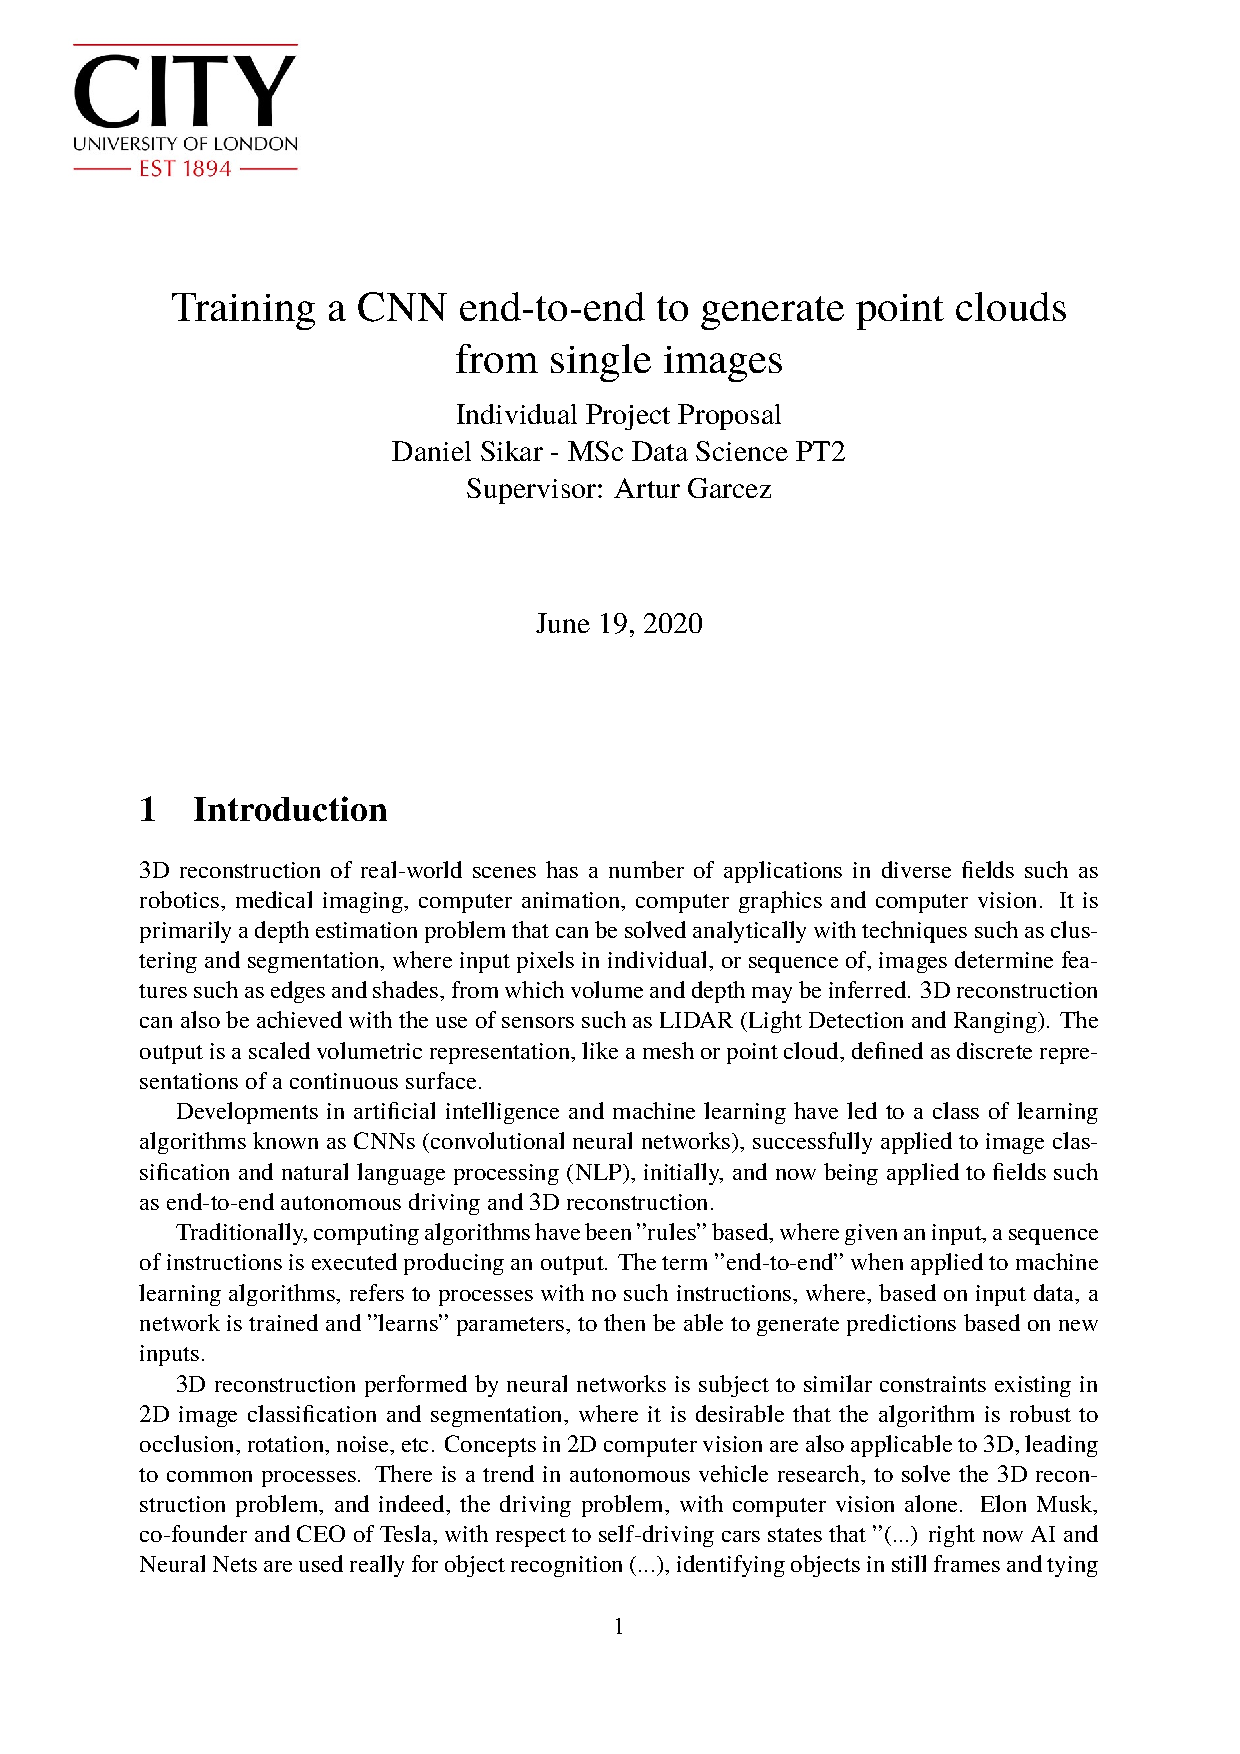
\includepdf[page={1-12}]{PointCloudCNN-DanielSikar-ResearchProjectProposal}


% Appendix A
% For referencing this appendix elsewhere, use \ref{AppendixA}
\chapter{Methods} % Main appendix title
\label{Appendix-methods} 

This appendix details procedures used to carry out the experiments

\section{conda}
\label{app:methods:Conda}

conda commands used in this project:
% Another good simplified reference
% https://docs.conda.io/projects/conda/en/latest/commands.html

\begin{verbatim}
# List conda environments
$ conda info --envs
# Activate conda - conda environment appears in parenthesis on command prompt
$ conda activate
# Deactivate conda
$ conda deactivate
# Create and activate environment
$ conda create --name cleargrasp
$ conda activate cleargrasp
# list modules
$ conda list
\end{verbatim}

\section{ClearGrasp Install}

For this project, ClearGrasp was originally deployed to an AWS (\cite{amazon2015amazon}) cloud EC2 server at the proof-of-concept stage, following the procedure described in \cite{cleargrasp-install2020}. For the actual work, using the Zivid One+ camera, ClearGrasp was deployed to a physical workstation: Dell Precison Tower 5810 with a 12-core Intel Xeon processor E5-1600 v3 and 32MB RAM. Given some software was already present, the procedure was simplified to:
\begin{verbatim}
# create conda environment
$ conda create --name cleargrasp
$ conda activate cleargrasp
# change python simlynk to point to v3.6.9
$ sudo ln -s /usr/bin/python3.6 /usr/bin/python
# install libraries
$ sudo apt-get install -y libhdf5-10 libhdf5-serial-dev libhdf5-dev libhdf5-cpp-11
$ sudo apt install -y libopenexr-dev zlib1g-dev openexr
$ sudo apt install -y xorg-dev  # display widows
$ sudo apt install -y libglfw3-dev
# clone repository
$ git clone git@github.com:Shreeyak/cleargrasp.git
$ cd cleargrasp
# download model checkpoints
$ wget http://clkgum.com/shreeyak/cleargrasp-checkpoints 
$ mv cleargrasp-checkpoints cleargrasp-checkpoints.zip
$ unzip cleargrasp-checkpoints.zip
$ mv cleargrasp-checkpoints data
# requirements
$ wget https://raw.githubusercontent.com/dsikar/cleargrasp/master/requirements_v2.txt
$ pip install -r requirements_v2.txt
# depth2depth compilation as per step 4 in https://github.com/Shreeyak/cleargrasp
# Install open3d
$ pip install open3d --no-cache-dir
# copy config file
$ cd eval_depth_completion/
$ cp config/config.yaml.sample config/config.yaml
# run evaluation
$ python eval_depth_completion.py -c config/config.yaml
\end{verbatim}




%\chapter{Results} % Main appendix title
\label{Appendix-results} % For referencing this appendix elsewhere, use 

%%%%%%%%%%%%%%%%%%%%%%%%%%%%%%%%%%%%%%%%%%%%%%%%%%%%%%%%%%%%%%%%%%%%%%%%%%%%%
% RUN XX - TEMPLATE - experiment log template
%%%%%%%%%%%%%%%%%%%%%%%%%%%%%%%%%%%%%%%%%%%%%%%%%%%%%%%%%%%%%%%%%%%%%%%%%%%%%
%\subsection{Run XX -  }
%\label{app_res:XX}
%\begin{verbatim}
%Commit:
%Model: 
%Outputs: 
%Dataset: 
%Command:
%Environment: 
%Comment: 
%\end{verbatim}



\end{appendices}
\end{document}  
